\section[GPS的计算模型]{GPS的计算模型\\Computational Models for GPS}
Before we study the general and rather complex code for Real Time Kinematic (RTK) processing, it can be reasonable to estimate the accuracy from pseudoranges alone and the improvements from phase observations. The purpose of Chapter 9 was to describe and investigate positioning using pseudoranges alone. That is the way in which most people know the usefulness of GPS, in the form of a simple hand-held receiver.

There we dealt with one-way code observations at receiver i on the LI frequency
from satellite k:
$$
Pseudorange \hspace{1cm} P_{1,i}^{k}=\rho_{i}^{k}+T_{i}^{k}+I_{i}^{k}+noise.
$$

The standard deviation of a C/A code observation is $\sigma_{code}$ = 3m and the standard deviation of the single point positioning, where one receiver tracks at least 4 satellites, is $\sigma \approx$ 10m.Using SBAS, a single receiver can obtain a standard deviation of $\sigma \approx$ 1-2m.

In easy4 we had single differences between receivers of code observations on L1:
$$
P_{1}=P_{1,i}^{k}-P_{1,j}^{k}
$$

This yields very little improvement in accuracy. In fact accuracy can be lost.

The big change in performance is achieved by observing both P-code and phase of the signal. This change is also reflected in the price. We may pay \$100 for the hand-held receiver, while the combined code and phase dual-frequency receiver costs \$ 20000.

The standard deviation $\sigma_{code}$ = 0.3 m of P-code observations is reduced to  $\sigma_{phase}$ =3 mm when phase observations are included. This improvement by a factor of 100 is remarkable and important. The phase observation of the carrier wave is
$$
Carrier phase  \Phi_{1,i}^{k}=\rho_{i}^{k}+T_{i}^{k}-I_{i}^{k}+\lambda_{1}N_{1}+ clock errors + multipath + noise
$$

and a single difference of these phase observations on L1 is
$$
\Phi_{1}=\Phi_{1,i}^{k}-\Phi_{1,j}^{k}
$$

Finally we make double differences of P-code observations from satellites k,l:
$$
P_{1,ij}^{kl}=(P_{1,i}^{k}-P_{1,i}^{l})-(P_{1,j}^{k}-P_{1,j}^{l})+noise
$$

The tropospheric delays can be modeled, the receiver clock offsets cancel, and the satellite clock offsets can be computed. The noise is left with ionospheric effects only:
$$
P_{1,ij}^{kl}=(\rho_{i}^{k}-\rho_{i}^{l})-(\rho_{j}^{k}-\rho_{j}^{l})+I_{ij}^{kl}
$$

For the phase $\Phi$, our observations may include integer ambiguities N:
$$
\Phi_{1,ij}^{kl}=(\rho_{i}^{k}-\rho_{i}^{l})-(\rho_{j}^{k}-\rho_{j}^{l})-I_{ij}^{kl}+\lambda_{1}((N_{1,i}^{k}-N_{1,i}^{l})-(N_{1,j}^{k}-N_{1,j}^{l}))+noise
$$

The precise differential position including code and phase observations, and with fixed ambiguities, achieves a standard deviation of $\sigma \approx$ 1-10mm.

\subsection{Differential GPS}

The idea behind differential GPS is to operate from a station with known coordinates. At this master site, we compute range corrections. Those corrections are transmitted to one or more roving receivers, to improve their positioning accuracy, see Figure 10.4. We restate this idea of differential positioning (DGPS) at nearby sites i and j:\\
- The short baseline allows us to use $I_{i}^{k}=I_{j}^{k}$ and $T_{i}^{k}=T_{j}^{k}$.\\
- Coordinates of the fixed site i are known.\\
- The unknowns are the coordinates x of the difference vector between site i and site j.\\
- We consider only L1 observations from one epoch, unless otherwise stated.

The following text and examples illustrate various models for Differential GPS.

\subsection{DGPS: Phase Observations}

We repeat the phase observation on L1 (in unit of length) between receiver i and satellite k
\begin{equation}
\Phi_{i}^{k}=\rho_{i}^{k}+cdt_{i}-cdt^{k}-I_{i}^{k}+T_{i}^{k}+\lambda_{1}N_{i}^{k}-\epsilon_{i}^{k}
\end{equation}

Atmospheric delays and satellite clock error combine into
\begin{equation}
E_{i}^{k}=cdt^{k}+I_{i}^{k}-T_{i}^{k}
\end{equation}

Then the linearized, one-way phase equations at receivers i and j are
$$
\Phi_{i}^{k}= cdt_{i}-E_{i}^{k}+\lambda_{1}N_{i}^{k}-\epsilon_{i}^{k}
$$
$$
\Phi_{j}^{k}= -(u_{j}^{k})^{T}x_{j}+cdt_{j}-E_{j}^{k}+\lambda_{1}N_{j}^{k}-\epsilon_{j}^{k}
$$

where
\begin{equation}
-(u_{j}^{k})^{T}=(\frac{X_{ECEF}^{k}-X_{i}}{\rho_{i}^{k}},\frac{Y_{ECEF}^{k}-Y_{i}}{\rho_{i}^{k}},\frac{Z_{ECEF}^{k}-Z_{i}}{\rho_{i}^{k}})
\end{equation}

\subsection{DGPS: Single Differences of Receivers}

Assume the position of receiver i is known.$P_{i}^{k}$ is related to the clock offset $cdt_{i}$ of the base receiver and can be applied as a range correction to $P_{j}^{k}$ of the rover(receiver j).Combining the models at i and j leads to the principle of differential GPS , using satellites k=1 to k=m to get accurate pseudorange $(P_{i}^{k})^{0}$ of the base station :
$$
\begin{bmatrix}
(P_{j \ obs}^{1}-(P_{j}^{1})^{0})-(P_{i \ obs}^{1}-(P_{i}^{1})^{0})\\
(P_{j \ obs}^{2}-(P_{j}^{2})^{0})-(P_{i \ obs}^{2}-(P_{i}^{2})^{0})\\
\vdots \\
(P_{j \ obs}^{m}-(P_{j}^{m})^{0})-(P_{i \ obs}^{m}-(P_{i}^{m})^{0})\\
\end{bmatrix}
=
\begin{bmatrix}
-(u_{j}^{1})^{0}&1\\
-(u_{j}^{2})^{0}&1\\
\vdots \\
-(u_{j}^{m})^{0}&1\\
\end{bmatrix}
\begin{bmatrix}
x_{j}\\y_{j}\\z_{j}\\cdt_{ij}
\end{bmatrix}
$$
Here $cdt_{j}-cdt_{i}$ comes from the difference of receiver clock offsets.\\

\textbf{Example 10.2} We have m-1 single frequency code observations
$$
\begin{bmatrix}
P_{ij}^{k2}\\
P_{ij}^{k3}\\
\vdots \\
P_{ij}^{km}
\end{bmatrix}
=\begin{bmatrix}
-(u_{j}^{k2})\\
-(u_{j}^{k3})\\
\vdots \\
-(u_{j}^{km})
\end{bmatrix}
x_{j}.
$$\\
With m = 4 satellites (3 double differences) we determine the three components of $x_{j}$.

Comparing the present observation equation for code with the observation equation for phase in Example 10.4 we may conclude that the phase observations formally have all ambiguities set to zero.

\begin{figure}
	\centering
	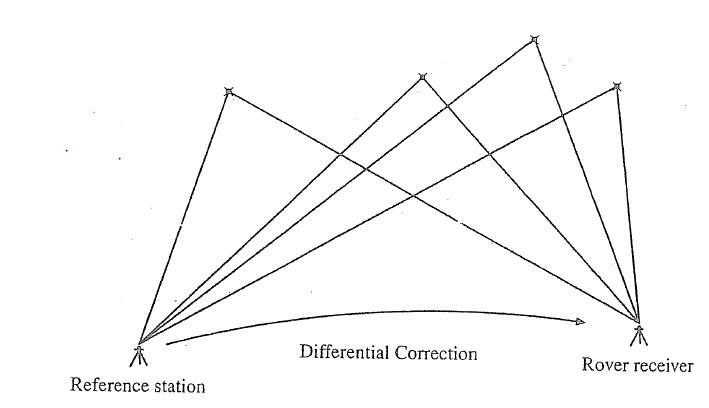
\includegraphics[width=0.4\linewidth]{TeX_files/Part03/chapter10/image/9-4}
	\caption{Principle for differential GPS: A known base station.}
	\label{fig:9-4}
\end{figure}

\subsection{DGPS: Double Differences of Receivers and Satellites}

We form differences between satellites k and i of single differences ( between receivers).
Satellite k will be the reference satellite:
\begin{equation}
\Phi_{ij}^{kl}=(\Phi_{j}^{l}-\Phi_{j}^{k})-(\Phi_{i}^{l}-\Phi_{i}^{k})
\end{equation}\\
The linearized observation equation is
$$
\Phi_{ij}^{kl}=-(u_{j}^{l}-u_{j}^{k})^{T}x_{j}+\lambda_{1}N_{ij}^{kl}+\epsilon_{ij}^{kl}
$$\\
Start with m single difference observations. Subtract the first one from the remaining m-1
observations to obtain m-1 double differences. At the same time remove one unknown:$\Phi_{ij}^{k}$ determines $cdt_{ij}$.

\textbf{Example 10.3} We have phase observations from m-1 non -reference satellites:
\begin{equation}
\begin{bmatrix}
\Phi_{ij}^{k2}\\
\Phi_{ij}^{k3}\\
\vdots \\
\Phi_{ij}^{km}
\end{bmatrix}
=\begin{bmatrix}
-u_{j}^{k2}&\lambda_{1}\\
-u_{j}^{k3}&           &\lambda_{1}\\
\vdots     &           &  &\ddots\\
-u_{j}^{km} & &\multicolumn{2}{c}{\raisebox{1.3ex}[0pt]{\Huge}} & \lambda_{1}
\end{bmatrix}
\begin{bmatrix}
x_{j}\\
N_{ij}^{k2}\\
N_{ij}^{k3}\\
\vdots\\
N_{ij}^{km}
\end{bmatrix}
\end{equation}\\
Both receiver and satellite oscillators have initial phase offsets $\Phi_{i}(t_{0})=\lambda\varphi_{i}(t_{0})$ and $\Phi^{k}(t_{0})=\lambda\varphi^{k}(t_{0})$.as in equation (10.2). So $N_{i}^{k}$ represents an integer number of cycles plus initial phase offsets. The offsets cancel by double differencing. Then the double differenced ambiguities $N_{ij}^{kl}$ are integers.

\textbf{Example 10.4} We have m-1 single frequency phase observations for two epochs:
$$
\begin{bmatrix}
\Phi_{ij}^{k2}(1)\\
\Phi_{ij}^{k3}(1)\\
\vdots \\
\Phi_{ij}^{km}(1)\\
\Phi_{ij}^{k2}(2)\\
\Phi_{ij}^{k3}(2)\\
\vdots \\
\Phi_{ij}^{km}(2)
\end{bmatrix}
=\begin{bmatrix}
-u_{j}^{k2}(1)&\lambda_{1}\\
-u_{j}^{k3}(1)&           &\lambda_{1}\\
\vdots     &           &  &\ddots\\
-u_{j}^{km}(1) & &\multicolumn{2}{c}{\raisebox{1.3ex}[0pt]{\Huge}} & \lambda_{1}\\
-u_{j}^{k2}(2)&\lambda_{1}\\
-u_{j}^{k3}(2)&           &\lambda_{1}\\
\vdots     &           &  &\ddots\\
-u_{j}^{km}(2) & &\multicolumn{2}{c}{\raisebox{1.3ex}[0pt]{\Huge}} & \lambda_{1}
\end{bmatrix}
\begin{bmatrix}
x_{j}\\
N_{ij}^{k2}\\
N_{ij}^{k3}\\
\vdots\\
N_{ij}^{km}
\end{bmatrix}
$$

The set contains 2m-2 observations and m+2 unknowns. If $m \geq 4$ we may determine all unknowns.

\textbf{Example 10.5} Combining (10.13) and (10.14) we introduce $\rho_{ij}^{*kl}=\rho_{ij}^{kl}-E_{ij}^{kl}$. In contrast to Example 10.4 we choose as unknowns $\rho_{ij}^{*kl}$ and $N_{ij}^{kl}$.
$$
\begin{bmatrix}
\Phi_{ij}^{k2}\\
\vdots \\
\Phi_{ij}^{km}
\end{bmatrix}
=\begin{bmatrix}
1&&& \lambda_{1}\\
& \ddots &&&& \ddots\\
& & 1 & & &&&\lambda_{1}\\
\end{bmatrix}
\begin{bmatrix}
\rho_{ij}^{*k2}\\
\vdots\\
\rho_{ij}^{*km}\\
N_{ij}^{k2}\\
\vdots\\
N_{ij}^{km}
\end{bmatrix}
$$\\
Satellites move, hence ranges change from epoch to epoch while integer ambiguities $N_{ij}^{kl}$ are constant. The estimation of ambiguities N is facilitated tremendously by including code observations.

\subsection{A Priori Covariance: Correlated Differences}

Suppose we are observing m satellites at a fixed epoch. We can set up m-1 linearly independent double differenced observations. Since those differences are correlated, the weight matrix (covariance) is no longer diagonal. Therefore this weight matrix must be handled with special care when the normal equations are formed. We now study this problem in detail.

Let the covariance matrix for the original phase observations be $\Sigma_{b}=\sigma_{0}^{2}I$. The observations are given with equal weight (equal variance) for phases. They are independent.The unit for the standard deviation $\sigma$ is length; as an example $\sigma$ = 0.01 m.

We assume all one-ways $\Phi_{i}^{k}$ are observed with the same variance $\sigma_{\Phi}^{2}$, and they are uncorrelated. For m observations $x=[\Phi_{i}^{1} \cdots \Phi_{i}^{m} \Phi_{j}^{1} \cdots \Phi_{j}^{m}]$ at sites i and j, the covariance matrix is $\Sigma_{x}=\sigma_{\Phi}^{2}I_{2m}$(unit matrix).

The vector s of single differenced phase observations has covariance matrix $2\sigma_{\Phi}^{2}I_{m}$
\begin{equation}
s=\begin{bmatrix}
\Phi_{ij}^{1}\\
\vdots\\
\Phi_{ij}^{m}
\end{bmatrix};
\Sigma_{s}=
\begin{bmatrix}
-I_{m}&I_{m}
\end{bmatrix}
\sigma_{\Phi}^{2}
\begin{bmatrix}
-I_{m}\\
I_{m}
\end{bmatrix}
=\sigma_{\Phi}^{2}
\begin{bmatrix}
2\\
&\ddots\\
\multicolumn{2}{c}{\raisebox{1.3ex}[0pt]{\Huge}}&2
\end{bmatrix}
\end{equation}\\
The vector $ d = Ds$ of double differenced phase observations has $\Sigma_{d}=D2\sigma_{\Phi}^{2}D^{T}$:
\begin{equation}
d=\begin{bmatrix}
\Phi_{ij}^{k2}\\
\vdots\\
\Phi_{ij}^{km}
\end{bmatrix}
=\begin{bmatrix}
-1&1\\
\vdots& & \ddots\\
-1&&&1
\end{bmatrix}s
=Ds;
\Sigma_{d}=\sigma_{\Phi}^{2}
\begin{bmatrix}
4&\cdots&2\\
\vdots&\ddots&\vdots\\
2&\cdots&4
\end{bmatrix}.
\end{equation}\\
The process of differencing leads to correlation!This covariance matrix $\Sigma_{d}$ has offdiagonal entries all equal to $2\sigma_{\Phi}^{2}$, because this is the variance of $\Phi_{ij}^{k}-\Phi_{ij}^{l}$.

In MATLAB this is\\
D = [ ones(m,1) - eye(m) - ones(m,1) eye(m)];\\
C = inv(D*D'); \% C will be eye(m-1))/2 - (ones(m-1))/(2*m)\\
W = chol(C); \% Cholesky triangular factorization C= W'*W\\
Winv = inv(W); \% multiplying by Winv decorrelates observations

The product $DD^{T}$ is the square matrix in (10.19); its diagonal entries are 4, all other entries are 2. Note that $DD^{T}$ is independent of the choice of reference satellite. Consequently C= $(DD^{T})^{-1}$ is independent of which column contains the -1s in D .

The matrix C =I/2-(ones) /2m is the weight matrix for these m - 1 correlated observations. If we want to decorrelate the observations, we compute the Cholesky factorization of C = $W^{T}W$ where W is upper triangular. The observations become uncorrelated when multiplied by $W^{-1}$, see Section 6.7.

\subsection{easy15}

A frequently asked question about GPS is: How accurate is a GPS - based position? The experienced GPS user knows that the big difference lies between using pseudoranges alone or including also carrier phases. We develop an idea of Misra \& Enge (2006).

To get a quantitative answer to this question, Kostas Dragunas recorded data simultaneously with a master and a rover receiver. He used two dual frequency receivers that store data in a binary format called the GPS Receiver Interface Language (GRIL).

The following message was sent to the receivers before the observation session:

dm
Em,,/msg/jps/GT,SI, R1,P1,R2,P2

Time of start was 481,860 seconds and the final epoch was at 484,395 seconds. So 2,535 synchronous epochs of observations were recorded with a one-second epoch interval.We deleted 95 epochs because of missing data at either the rover or the master, or repeated estimation of ambiguities . This makes a continuous record of about 42 minutes .

The original observations were modified in several ways: After each ephemeris, the master receiver issued two subsequent P2 messages (full P/L2 carrier phases, binary identical). The rover receiver erroneously sometimes issued two subsequent GPS Time(GT) messages��wn and tow (binary identical).

easy15 assumes data arriving in real-time from the two receivers. In reality, we read from two files, 19jan07m.log and 19jan07r.log, containing a mixture of observations and ephemerides. The baseline between receivers is about 1509.3 m.

The actual reading of the log-files is done by the readGrilM and readGrilR functions.We are using two similar codes for each log -file to avoid too much bookkeeping about the location of binary data. A typical reading contains time of week, tracked satellites (identified by pseudorandom noise codes or PRNs), and observed pseudorange and carrier phas -e on the two frequencies.

The reading is complicated by the fact that new ephemerides may appear at any time between the observations. The ephemerides are stored in a global matrix EPH . When a new version of an ephemeris arrives , it overwrites the old one.

Since we read from two stored files, we have to determine the first epoch common to both receivers. Next we determine the number of tracked PRNs at both master and rover sites for which we know the ephemerides.

When the number of common PRNs is four or more, we compute the master position using the recposRTK function, and all elevation angles as seen at the master position. We delete low-elevation PRNs and select a reference PRN. Next all observations are rearranged so that master and rover data match each other-the sequence of PRNs in the master and rover receivers are likely to be different. Ambiguities are estimated using Clyde Goad ��s method as described in Section 10.6.

New PRNs at the master and rover most often occur at different epochs. Hence, we need to omit the observations from one receiver until the PRN appears with complete data at both receivers. We recompute the master position with good PRNs and find the ellipsoidal height hi needed for the later computation of tropospheric delay.

We choose a Kalman filter where the state vector x contains the baseline components (x,y,z). We initialize the covariance matrices $\Sigma_{e,k}$ and $\Sigma_{\epsilon,k}$ and $P_{0|0}$ for the observations and system equations and state vector.

\textbf{Remark 10.1} A Kalman filter and its innovation vector may run smoothly and the baseline components may still be wrong. A correct ambiguity estimation leads to excellent estimates of the baseline. Incorrect ambiguities definitely lead to incorrect baselines, while the filter makes biased and slow corrections striving at the correct values.

Next we read one epoch of data in the master and rover files, prepare double differences,correct for tropospheric delays, and then set up the innovation vector $b-Ax$.We update the filter, plot the result in an open figure window and proceed to the next epoch.

\begin{figure}
	\centering
	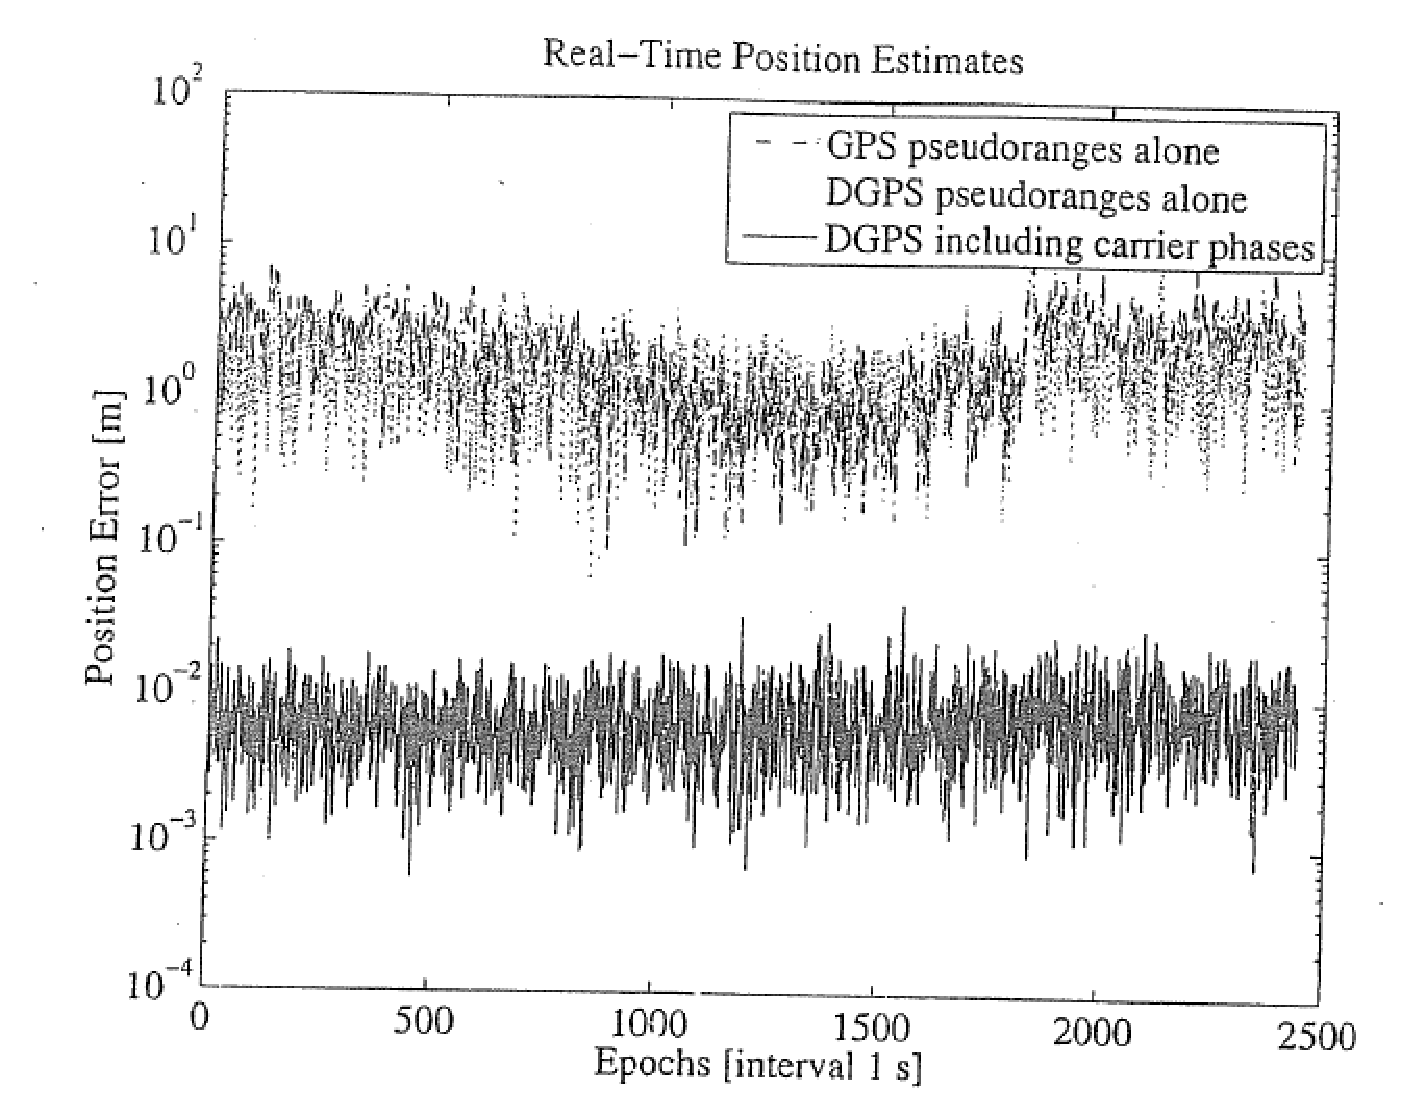
\includegraphics[width=0.4\linewidth]{TeX_files/Part03/chapter10/image/9-5}
	\caption{A stand-alone position and a differential position based on pseudoranges alone have position errors of a few meters,while adding carrier phase observations brings the position error down to the centimeter-level or below.}
	\label{fig:9-5}
\end{figure}

This code is the closest we get to a real-time kinematic (RTK) code without having two receivers connected directly to the laptop��s com port. If that laptop configuration can be achieved , then a user may set up the ports using the I/O facility. For one port the following code reads a data stream from the receiver into the file legacy.tex:

s = serial('COM2');

s.OutputBufferSize = 512;

s.InputBuffersize = 50000;

fopen(s);

s. BaudRate = 9600;

set(s,'TimeOut',1 );

s.RecordMode = 'index';

s.Record Detail = 'verbose';

s.RecordName = 'legacy.tex';

Figure 10.5 illustrates two levels of real - time positioning accuracy from GPS, with position errors ranging from several meters to centimeters. The norm of the error is plotted for observations taken at one-second intervals for about 42 minutes.

The raw L1 pseudorange accuracy is typically a few meters. Access to concurrent pseudo -range observations from a GPS master receiver (at a known location ) does not reduce the errors significantly; possibly it eliminates some common trends in the positions.

\begin{figure}
	\centering
	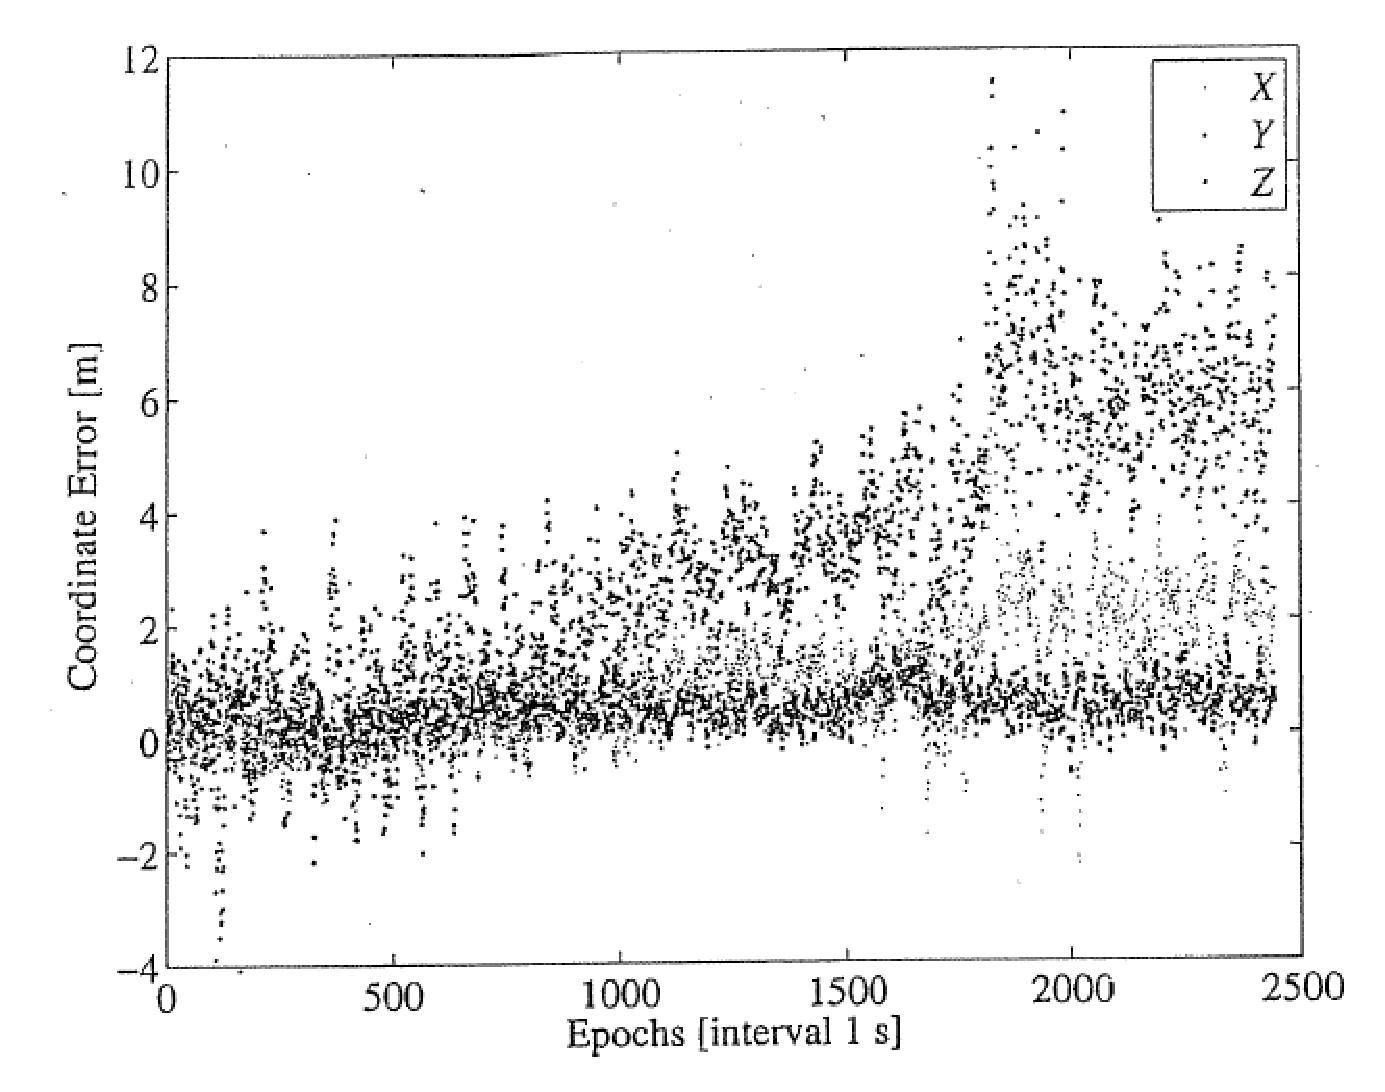
\includegraphics[width=0.4\linewidth]{TeX_files/Part03/chapter10/image/9-6}
	\caption{A stand-alone position and a differential position based on pseudoranges alone have position errors of a few meters,while adding carrier phase observations brings the position error down to the centimeter-level or below.}
	\label{fig:9-6}
\end{figure}

The full potential of the observational data is exploited by including both pseudoranges
and carrier phases, to obtain position estimates at centimeter-level or better.

Figure 10.6 shows the variation over 42 minutes , for master station coordinates as computed from pseudoranges alone. Typically the X and Y coordinates show a lesser variation than the Z coordinate (for Aalborg,Denmark).